\documentclass[12pt, a4paper, twoside, notitlepage]{book}
\usepackage[portuguese]{babel}
\usepackage[latin1]{inputenc}
\usepackage[T1]{fontenc}
\usepackage{graphicx, lastpage}
\usepackage{subfigure}
\usepackage{fancyvrb}
\usepackage{color}
\usepackage{float}
\usepackage{url}
\usepackage{listings}


\newcommand{\programa}[1]{\texttt{#1}}

%cores
\definecolor{cinza}{rgb}{0.8,0.8,0.8} %fundo do codigo

\title{%
{\Huge Sebenta}\\%
de\\%
Processing\\%
{\small a.k.a.: Programação para Artistas, Artistas Digitais, Pseudo-Artistas/Digitais, e Todos os Outros... (usando o Processing)}\\%
}
\author{\copyright Jorge Cardoso}

\begin{document}
\lstset{language=java, basicstyle=\small\ttfamily, breaklines=true, numbers=left, backgroundcolor=\color{cinza}}
%\lstset{language=Java,basicstyle=\footnotesize\ttfamily, breaklines=true, numbers=left}
\lstset{moredelim=[is][\itshape\bfseries]{/**/}{/**/}}%
\renewcommand{\lstlistingname}{Exemplo}
\renewcommand{\lstlistlistingname}{Exemplos}

\frontmatter
%%%%%%%%%Pagina de Titulo%%%%%%%%%%%%%
\maketitle
\thispagestyle{empty}
\vfill
%\begin{r}
\noindent
Universidade Católica Portuguesa -- Centro Regional do Porto - Foz\\
Escola das Artes\\
Curso de Som e Imagem\\
%\end{center}
\vfill
\begin{center}
Built with \LaTeX
\end{center}
\clearpage
\setcounter{page}{0}
\thispagestyle{empty}
\clearpage
\tableofcontents
\clearpage
\lstlistoflistings

%\include{Agradecimentos/dedicatoria}
%\cleardoublepage
\include{Agradecimentos/Agradecimentos}
\cleardoublepage

\mainmatter

\part{O Básico}
\chapterimage{band1.png}
\chapter{Introdução - o que é programar? }

Este capítulo pretende dar apenas uma visão geral do que significa programar um computador. O leitor mais ávido por começar a experimentar pode avançar para o próximo capítulo.

\section{Programação}
``Programar'', no contexto deste manual, significa definir um conjunto de instruções que irão ser executadas por uma máquina. No entanto, pode ser instrutivo fazermos a analogia máquina--pessoa, i.e., pensarmos em exemplos do nosso quotidiano e imaginarmo-nos a ``executar um programa'', para ilustrar alguns conceitos associados à programação de computadores.

%Estas instruções, ou passos, não são mais do que ``comandos'' que a máquina ou pessoa deve executar para chegar ao objectivo final. 


%Se estivermos a definir um programa para ser seguido por um ser humano, as instruções que lhe damos são muito diferentes das
%instruções que dariamos a um computador. 
Por exemplo, o seguinte programa para abrir a porta quando alguém bate seria facilmente seguido por uma pessoa%
\footnote{Os programas mostrados nesta secção utilizam uma sintaxe livre, i.e.%
, não estão escritos numa linguagem de programação particular. Estão escritos em pseudo-código, ou seja, uma linguagem utiliza apenas para comunicar programas entre 
pessoas. Estes programas não podem ser executados num computador, servem apenas para efeitos de exemplificação dos conceitos básicos.}%
:
\begin{lstlisting}[caption=Programa ``Atender a porta'', label=exe:atenderPorta]
esperar que alguém bata à porta.
levantar da cadeira.
dirigir-se à porta.
abrir a porta.
perguntar em que pode ajudar.
\end{lstlisting}

Este primeiro exemplo serve para ilustrar algumas características da programação.
Primeiro, a ordem das instruções é extremamente importante; as linhas estão numeradas para dar relevância a esse facto. O programa não funcionaria se a execução trocasse a ordem de uma das instruções para, por exemplo:

\begin{lstlisting}[caption=Programa ``Atender a porta'' com instrução trocada, label=exe:atenderPortaOrdemTrocada]
levantar da cadeira.
dirigir-se à porta.
abrir a porta.
esperar que alguém bata à porta.
perguntar em que pode ajudar.
\end{lstlisting}

Segundo, as instruções são escritas na forma imperativa. Ao programar podemo-nos imaginar a dar ordens a quem executa o programa.

O Exemplo~\ref{exe:atenderPorta} ilustra ainda uma outra característica dos programas de computador: a entrada e saída de dados. Um programa não seria muito útil se não produzisse nada que pudesse ser utilizado pela pessoa que o executa. A saída de um programa pode tomar várias formas, e.g., números no ecrã, uma folha de papel na impressora, efeitos visuais, som, actuação física de motores de um robô, etc. Da mesma forma, a maioria dos programas permitem que o utilizador introduza, de alguma forma, dados que serão manipulados por esse programa. A forma mais típica de introdução de dados é através do rato e teclado, mas um programa pode obtê-los através de várias formas, como leitura de um ficheiro previamente escrito, leitura de sensores ligados ao computador, imagens de cameras web, áudio do microfone, etc. 



%O programa anterior seria facilmente executado por uma pessoa, mas não por um computador. O programa é demasiado ambíguo para ser executado por uma máquina. Por exemplo, o que aconteceria se a sala tivesse várias portas? Logicamente, uma pessoa iria atender a porta de onde veio o som... mas uma máquina não tem este tipo de compreensão. A instrução 
%\begin{verbatim}
%3 - dirigir-se à porta
%\end{verbatim}
%é demasiado vaga para uma máquina -- é necessário especificar qual a porta para onde devemos dirigirmo-nos. Os programas de computador necessitam, por isso, de um conjunto de instruções precisas que o computador (ou melhor, o processador do computador) saiba executar.



%\section{Algoritmos}
%Normalmente fazemos a distinção entre \emph{algoritmo} e \emph{programa}. Estes dois conceitos estão intimamente relacionados mas têm significados ligeiramente diferentes:
%\begin{description}
%\item[Algoritmos]
%Um algoritmo%
%\footnote{A palavra algoritmo tem origem no nome do matemático persa Al-Khwarizmi - 780-850.}
%é um ``conjunto de regras e operações que permitem resolver, num número finito de etapas, um problema''\cite{infopedia}.
%
%\item[Programa]
%Um programa de computador é um ``conjunto completo de instruções, em linguagem de código, que indica ao computador, passo a passo, como determinada tarefa deverá ser executada''\cite{infopedia}.
%\end{description}
%
%Dito de forma mais simples, um programa é uma implementação concreta de um algoritmo.
%
%É útil fazer esta distinção porque a definição de um algoritmo permite-nos comunicar a resolução de um problema sem nos preocuparmos com os detalhes sintácticos ou semânticos de uma determinada linguagem de programação.
%
%Normalmente os algoritmos são especificados em linguagem natural, i.e.%
%\footnote{\emph{i.e.} -- significa \emph{isto é} (do latim, \emph{id est}).}%
%, em Português, ou em pseudo-código -- uma linguagem intermédia entre a natural e uma linguagem de programação. 
%Os programas são escritos numa determinada linguagem de programação, e.g.%
%\footnote{\emph{e.g.} -- significa \emph{por exemplo} (do latim, \emph{exempli gratia}).}%
%, Processing, C, Java, ActionScript, PHP, etc.


\section{Como Funciona o Processador de um Computador}


\section{História Resumida das Linguagens de Programação}


\section{Linguagens de Programação}
Existem várias linguagens que podemos utilizar para programar. Algumas apenas funcionam em determinados ambientes, por exemplo, o ActionScript é uma linguagem para programar Flash, ou seja apenas funciona no programa Macromedia Flash.
O PHP, por outro lado, serve apenas para programar páginas web, i.e., não podemos criar um programa com janelas e botões em PHP.
A linguagem C, por outro lado é uma linguagem mais tradicional -- serve para escrever programas que correm directamente no computador.

Apenas como curiosidade, aqui fica uma pequena lista das linguagens de programação mais comuns:
\begin{description}
\item[Processing]
Uma linguagem de programação baseada na linguagem Java. Criada para simplificar a programação em Java e para servir como ferramenta para artistas digitais e para o ensino da programação.

\item[Java] 
Uma linguagem de programação criada em 1995 como o objectivo de permitir a criação de programas que possam ser executados em várias plataformas sem modificação. A sua utilização tornou-se mais conhecida através das \emph{applets} -- pequenos programas que podem ser executados num browser. Os programas escritos em Java são compilados num código máquina virtual que é depois (aquando da execução do programa) transformado em código máquina real.

\item[C/C++] 
Uma das linguagens mais utilizadas e mais antigas no mundo. A sintaxe é muito parecida com a do Java (a sintaxe do Java foi inspirada no C). Um programa escrito em C tem de ser compilado para código máquina antes de poder ser executado.

\item[PHP] 
O PHP não é bem uma linguagem de programação, no sentido em que não permite a criação de programas de computador como os entendemos geralmente. O PHP não permite criar um programa (com janelas, menus, botões, etc) para ser executado num computador pessoal. Esta linguagem é destinada à criação de páginas Web e, por isso, os programas escritos em PHP não são compilados em código máquina. Um programa PHP é executado pelo servidor Web; por esta razão diz-se que o PHP é uma linguagem de \emph{scripting}%
\footnote{Uma linguagem de scripting é uma linguagem em que os programas precisam de um outro programa para executar. O PHP precisa de um servidor Web para executar o seu código, por exemplo. O ActionScript precisa do Flash Player para correr...}

\item[ActionScript]
Uma linguagem de scripting utilizada para programar em Flash.

\item[VisualBasic]
Uma linguagem de programação para o sistema Windows, introduzida pela Microsoft. 

\end{description}

\subsection{Compilar e Executar}
Nos primórdios da computação, a programação de um computador era feita usando instruções entendidas directamente pelo computador. Estas instruções são designadas por código máquina. Computadores diferentes (com processadores diferentes) possuem conjuntos de instruções diferentes, pelo que um programa escrito em código máquina apenas executa num determinado tipo de computador. 
A programação em código máquina era muito trabalhosa e propícia a erros (as instruções são compostas por '0's e '1's), pelo que era necessário pessoal altamentente especializado para efectuar a tarefa de programação de um computador.

À medida que a área avançou apareceram novas formas de programar: em vez de escrevermos um programa em código máquina, por que não escrever numa linguagem mais próxima da linguagem natural e fazer um programa que converta entre a linguagem natural (a usada pelo programador) e a linguagem máquina? Foi então que surgiram as primeiras linguagem de programação de alto nível%
\footnote{Uma linguagem de alto nível é uma linguagem com uma sintaxe mais próxima da linguagem natural do que a linguagem em código máquina.}%
.

Associado às linguagens de alto nível está um tipo de programa especial: o compilador. O compilador não é mais do que um programa que converte o programa escrito pelo programador em linguagem de alto nível para código máquina de forma a poder ser executado pelo computador. O programa escrito pelo programador é designado por \emph{código fonte}.


\section{Lógica e Sintaxe}
O código fonte de um programa pode ser visto de duas perspectivas: da lógica do programa; e da sintaxe.

Uma determinada linguagem de programação é definida principalmente pela sua sintaxe, ou seja pelas regras que definem o que é um programa bem escrito. Da mesma forma que a sintaxe da língua Portuguesa define as regras de construção de frases, também a sintaxe da linguagem de programação define as regras de construção de um programa escrito nessa linguagem. Por exemplo, a frase ``O João foi às compras.'', está de acordo com as regras, mas ``O João às foi compras.'', não está. Apesar de o significado de ambas as frases ser óbvio e idêntico: o João foi às compras, a segunda quebra as regras da construção de frases em Português.

A lógica de um programa equivale ao seu significado. No exemplo anterior a lógica (significado) da frase era óbvia, mas estava mal construida. Também um programa pode estar logicamente correcto, mas sintacticamente incorrecto. Um programa sintacticamente incorrecto não pode ser compilado (os compiladores não são ``suficientemente inteligentes'' para perceberem o significado do programa de modo a corrigirem a sintaxe). Os erros sintácticos são facilmente detectados pelo compilador.
De forma inversa, um programa pode estar sintacticamente correcto, mas logicamente não. Nestes casos, o programa é compilado e executado, mas o resultado não é o que o programador estava à espera. Estes erros são mais difíceis de detectar!




\section{Nível de Detalhe}
Quando escrevemos um programa em Português a que nível de detalhe devemos ir na especificação das instruções?
Por exemplo, se quisermos escrever um programa para uma pessoa mudar um pneu de um carro podemos ter algo como o seguinte:
\begin{verbatim}
1 - sair do carro.
2 - abrir a mala do carro.
3 - tirar pneu sobresselente.
4 - tirar macaco.
5 - tirar chave.
6 - desapertar ligeiramente as porcas do pneu.
7 - colocar o macaco debaixo do carro.
8 - dar \'a manivela até o pneu ficar suficientemente levantado.
9 - desapertar as porcas na totalidade.
10 - retirar o pneu furado.
11 - colocar o pneu novo.
12 - apertar as porcas.
13 - baixar o carro.
14 - retirar o macaco.
15 - apertar bem as porcas.
16 - guardar chave.
17 - guardar macaco.
18 - guardar pneu furado.
\end{verbatim}

Mas, estamos a assumir que a pessoa sabe fazer uma série de coisas, como sair do carro, abrir a mala, etc.
Cada um dos passos do nosso programa anterior pode ele mesmo ser um programa em si. Por exemplo sair do carro:
\begin{verbatim}
1 - desligar o carro.
2 - apertar o travão de mão.
3 - retirar o cinto de segurança.
4 - retirar a chave da ignição.
5 - abrir a porta.
6 - sair.
7 - fechar a porta.
\end{verbatim}

Então, a que nível de detalhe deveremo ir quando estamos a escrever um programa? No caso de um programa para ser executado por uma pessoa, devemos descer ao nível de detalhe suficiente para a pessoa conseguir executar cada passo. Obviamente, isto depende da tarefa e da pessoa.

No caso de um programa de computador, o problema não se coloca a este nível. Ao utilizarmos uma determinada linguagem de programação, estamos automaticamente limitados às instruções mais básicas fornecidas por essa linguagem. Por exemplo, no caso do desenho num ecrã, algumas linguagens apenas possuem instruções para desenhar um pixel numa determinada posição do ecrã. Neste caso, se quisermos fazer uma programa para desenhar uma linha vertical teriamos de fazer algo do género:
\begin{verbatim}
1 - desenhar pixel na primeira posicao da linha.
2 - avancar um pixel na vertical.
3 - desenhar um pixel na nova posicao.
4 - repetir o passo 2 até chegar ao final da linha.
\end{verbatim}

Outras linguagens têm instruções para desenhar linhas, pelo que o programa anterior se resumiria a uma única instrução:
\begin{verbatim}
1 - desenhar linha vertical.
\end{verbatim}

Ou seja, quando programamos um computador temos de utilizar as instruções fornecidas pela linguagem que estamos a utilizar. Daí que algumas linguagens sejam mais aplicadas nalguns tipos de programas -- possuem instruções que facilitam a escrita de determinados programas.

No entanto, o problema do nível de detalhe coloca-se sob outra perpectiva quando programamos um computador. Todas as linguagens permitem-nos definir as nossas próprias instruções compostas por sequências maiores de instruções básicas. Por exemplo, no caso da linguagem que apenas permite desenhar um pixel numa posição do ecrã, poderiamos compor uma nova instrução: \texttt{desenharLinhaVertical}, à custa dos passos do nosso programa exemplo. Assim, sempre que quisessemos desenhar uma linha vertical no ecrã bastava usar a nova instrução:
\begin{verbatim}
1 - desenharLinhaVertical.
\end{verbatim}

Quando escrevemos um programa devemos pensar em agrupar conjuntos de instruções de forma a termos ao nosso dispor instruções que efectuam vários passos de cada vez. 
A questão agora é saber que instruções agrupar. Novamente, não há uma resposta única. Depende do programa. É uma questão de experiência (e, às vezes, de estilo do programador).

\section{Conceitos Básicos de Um Programa}
Quando criamos programas, ou, de forma mais genérica, quando pensamos em algoritmos, existem alguns conceitos fundamentais que são comuns a todos eles: \emph{memória}, \emph{selecção} e \emph{iteracção}.

\begin{description}
\item[memória]\footnote{O conceito de memória será aprofundado no Capítulo~\ref{cap:memoria}.}
A memória é o que permite ao nosso programa guardar dados temporários ou intermédios para serem utilizados mais tarde.
Por exemplo, se pretendessemos criar um programa para calcular os pontos da equipa do FCP no campeonato fariamos algo do género:
\begin{verbatim}
1 - ler jogosGanhos.
2 - ler jogosEmpatados.
4 - pontos = jogosGanhos * 3 + jogosEmpatados.
5 - escrever pontos.
\end{verbatim}
No programa anterior a instrução \texttt{ler}, coloca numa \emph{variável} um valor fornecido pelo utilizador. Uma variável
é a memória do nosso programa. É como uma gaveta com nome, na qual podemos guardar valores para mais tarde utilizar.
O programa anterior precisa de guardar os valores do número de jogos ganhos e empatados para poder efectuar a operação matemática que devolve o número de pontos no campeonato. O resultado desse cálculo, é, ele mesmo, colocado também numa ``gaveta'' para posterior utilização. Uma vez colocados na ``gaveta'' (variável), os dados podem ser consultados em qualquer altura (ponto de execução) do nosso programa. 

\item[selecção] \footnote{O conceito de selecção será aprofundado no Capítulo~\ref{cap:seleccao}.}
O conceito de \emph{selecção} está associado ao caminho executado pelo nosso programa. Um programa pode ser visto como uma árvore: a execução começa por um ponto comum -- o tronco, e, à medida que o programa executa, pode percorrer um ramo ou outro, dependendo das circunstâncias no momento da execução.
Por exemplo, no programa seguinte:
\begin{verbatim}
1 - ler jogosGanhosFCP.
2 - ler jogosEmpatadosFCP.
3 - ler jogosGanhosSLB.
4 - ler jogosEmpatadosSLB.
5 - pontosFCP = jogosGanhosFCP * 3 + jogosEmpatadosFCP.
6 - pontosSLB = jogosGanhosSLB * 3 + jogosEmpatadosSLB.
7 - se pontosFCP > pontosSLB então
    8 - escrever "O FCP está à frente do SLB".
9 - senão
    10 - escrever "O SLB está à frente do FCP".     
\end{verbatim}

existe um ``tronco'' comum a todas as execuções do programa -- as linhas de 1 a 7.
No entanto, consoante a pontuação de uma e outra equipa, o programa pode percorrer o ramo 8 -- se o FCP tiver mais pontos que o SLB, ou o ramo 10 -- se o SLB tiver mais pontos que o FCP.
A linha 7 -- \texttt{se pontosFCP > pontosSLB}%
\footnote{O símbolo ``>'' significa ``maior do que''.}
\emph{selecciona} o ramo%
\footnote{As linhas 8 e 10 estão \emph{indentadas}, isto é, escritas mais à direita, para facilitar a leitura do programa. Desta forma é óbvio que o ramo 8 corresponde à condição ser verdadeira e o 10 à condição falsa. Caso contrário, não seria facilmente perceptível que o programa contém ramos.}
a executar no programa.

\item[iteracção]\footnote{O conceito de iteracção será aprofundado no Capítulo~\ref{cap:iteraccao}.}
A maior parte dos programas que escrevemos contêm partes que são repetidas várias vezes. Por exemplo, se quisermos calcular as pontuações de todas as equipas do campeonato, poderiamos construir um programa do género:
{\small
\begin{verbatim}
1 - ler jogosGanhosEquipa1.
2 - ler jogosEmpatadosEquipa1.
3 - pontosEquipa1 = jogosGanhosEquipa1 * 3 + jogosEmpatadosEquipa1.
4 - escrever pontosEquipa1.
5 - ler jogosGanhosEquipa2.
6 - ler jogosEmpatadosEquipa2.
7 - pontosEquipa2 = jogosGanhosEquipa2 * 3 + jogosEmpatadosEquipa2.
8 - escrever pontosEquipa2.
9 - ler jogosGanhosEquipa3.
10 - ler jogosEmpatadosEquipa3.
11 - pontosEquipa3 = jogosGanhosEquipa3 * 3 + jogosEmpatadosEquipa3.
12 - escrever pontosEquipa3.
...
68 - ler jogosGanhosEquipa18.
70 - ler jogosEmpatadosEquipa18.
71 - pontosEquipa18 = jogosGanhosEquipa18 * 3 + jogosEmpatadosEquipa18.
72 - escrever pontosEquipa18.
\end{verbatim}}
Neste programa, para calcular a pontuação de 18 equipas, precisamos de 72 linhas de código! No entanto, se olharmos bem, as linhas são muito parecidas -- as primeiras 4 linhas repetem-se ao longo do programa. Existe uma estrutura que nos permite economizar linhas de código: o \emph{ciclo}. Vejamos o seguinte programa:
{\small
\begin{verbatim}
1 - i = 1.
2 - enquanto i == 18 fazer
    3 - ler jogosGanhosEquipa.
    4 - ler jogosEmpatadosEquipa.
    5 - pontosEquipa = jogosGanhosEquipa * 3 + jogosEmpatadosEquipa.
    6 - escrever pontosEquipa.
    7 - i = i + 1.
\end{verbatim}}
Neste caso, colocamos as 4 linhas repetidas do programa anterior dentro daquilo a que chamamos \emph{ciclo} -- uma estrutura repetitiva de código (iteractiva)%
\footnote{Não confundir \emph{iteractiva} -- que se repete; com \emph{interactivo} -- que permite a troca de informação entre sistema e utilizador.}%
. 
Basicamente, o programa utiliza uma variável para contar as equipas que já calculámos: a variável \texttt{i}. Enquanto 
codificação.

\end{description}



\section{Exercícios}

\subsection{Resolvidos}

\begin{enumerate}
	\item \label{exe:1_1} Escreva um programa em linguagem natural para ligar os computadores de uma sala de aulas. Escreva o programa para ser seguido por uma pessoa. O programa deve ter pelo menos uma tomada de decisão.
	
	\item \label{exe:1_2} Baseando-se no programa que escreveu no ponto anterior, substitua cada instrução desse programa por um conjunto de instruções mais detalhadas.
	
	\item \label{exe:1_3} 
\end{enumerate}

\subsection{Para Resolver}
\begin{enumerate}
\item 
Pensar num programa que possa ser facilmente implementado por um colega seu na sala de aula. Escrever esse programa.  O programa deve ter mais de 10 instruções, deve ter pelo menos uma estrutura de selecção ou iteracção e deve poder ser executado em menos de 5 minutos.

\item Escreva o programa anterior com um nível de detalhe maior.

\item (Tentar) Agrupar as novas instruções em conjuntos de instruções maiores e diferentes do original.
\end{enumerate}

\subsection{Resolução dos Exercícios Resolvidos}

{\footnotesize
\subsubsection*{Exercício \ref{exe:1_1}}
\begin{verbatim}
Programa Ligar os Computadores da Sala

1 - Dirigir-se ao primeiro computador.
2 - Carregar no botão de ``power'' do computador.
3 - Carregar no botão de ``power'' do monitor.
4 - Se computador não ligou
    5 - Verificar cabos de alimentação
    6 - Repetir o passo 2.
7 - Verificar se há mais computadores     
8 - Se houver mais computadores então
    9 - Dirigir-se ao computador seguinte.
    10 - Repetir o passo 2.
11 - Senão
    12 - Termina.    
\end{verbatim}}
\paragraph{Notas}
Este programa funciona apenas se determinadas condições se verificarem. Uma vez que 
não colocámos instruções para verificar se o computador já estava ligado, caso
isso aconteça o computador será desligado. Para o programa funcionar como
pretendido é necessário que todos estejam desligados.


\subsubsection*{Exercício \ref{exe:1_2}}
{\footnotesize
\begin{verbatim}
Programa Ligar os Computadores da Sala (mais detalhe)

1 - Dirigir-se ao primeiro computador.
2 - Verificar se o computador está desligado.
3 - Se o computador estiver desligado então
    4 - Identificar botão de ``power'' do computador.
    5 - Levantar a mão e esticar o dedo indicador.
    6 - Pressionar o botão de ``power'' do computador.
7 - Verificar se o monitor está desligado.
8 - Se o monitor estiver desligado então
    9 - Identificar botão de ``power'' do monitor.
    10 - Levantar a mão e esticar o dedo indicador.
    11 - Pressionar o botão de ``power'' do monitor.
12 - Se computador não ligou
    13 - Verificar cabos de alimentação do computador.
    14 - Verificar os cabos de alimentação do monitor.
    15 - Repetir o passo 3.
16 - Verificar se há mais computadores     
17 - Se houver mais computadores então
    18 - Dirigir-se ao computador seguinte.
    19 - Repetir o passo 2.
20 - Senão
    21 - Termina.    
\end{verbatim}}

\subsubsection*{Exercício \ref{exe:1_3}}
{\footnotesize
\begin{verbatim}
Programa Ligar os Computadores da Sala (mais detalhe)

Instrução Ligar o Computador:
1 - Verificar se o computador está desligado.
2 - Se o computador estiver desligado então
    3 - Identificar botão de ``power'' do computador.
    4 - Levantar a mão e esticar o dedo indicador.
    5 - Pressionar o botão de ``power'' do computador.
6 - Fim Instrução    

Instrução Ligar o Monitor:
1 - Verificar se o monitor está desligado.
2 - Se o monitor estiver desligado então
    3 - Identificar botão de ``power'' do monitor.
    4 - Levantar a mão e esticar o dedo indicador.
    5 - Pressionar o botão de ``power'' do monitor.
6 - Fim Instrução

1 - Dirigir-se ao primeiro computador.
2 - [Ligar o Computador]
3 - [Ligar o Monitor]
12 - Se computador não ligou
    13 - Verificar cabos de alimentação do computador.
    14 - Verificar os cabos de alimentação do monitor.
    15 - Repetir o passo 2.
16 - Verificar se há mais computadores     
17 - Se houver mais computadores então
    18 - Dirigir-se ao computador seguinte.
    19 - Repetir o passo 2.
20 - Senão
    21 - Termina.
\end{verbatim}}
\include{020-processando}
\include{030-variaveis}
\include{040-condicionais}
\include{050-iteraccao}
%%modulos
%
%%\chapter{Matriz - A Sequela}
%%%vectores e matrizes
\include{060-funcoes}
\include{065-classes}
\include{070-comentarios}
\include{080-pseudocodigo}
%%%\include{095-mvc}
%
%\part{O Avançado}
%\chapter{Eu Cá, Tu Lá... (Interacção)} \label{cap:interaccao}
A maioria dos programas que construímos necessitam que o utilizador
interaja com o computador. Por exemplo, se quisermos que o utilizador escolha uma entre várias opções, se pretendermos obter um texto, etc.

Existem várias formas de obter dados do utilizador. Para além do teclado e do rato, é possível utilizar sensores, camâras \emph{web}, etc. Este capítulo, no entanto, dedica-se apenas à interacção através do teclado e do rato do computador.

\section{O Rato} 
A informação que podemos obter do rato do computador resume-se à sua localização espacial (a posição (x, y) do ponteiro do rato) e o estado dos botões.

O ponteiro do rato é representado internamente, no computador, como um ponto num sistema de coordenadas bidimensional (um ponto com coordenadas (x, y)). O sistema de coordenadas tem origem (0, 0), no canto superior esquerdo da janela do Processing. A Figura~\ref{fig:coordinatesrato} exemplifica isto.
\begin{figure}
	\centering
		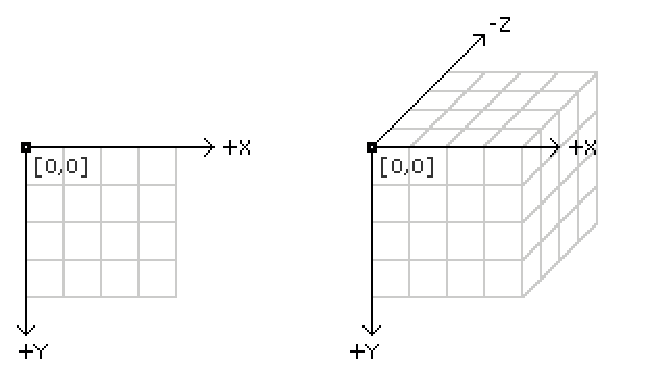
\includegraphics{images/coordinates.eps}
	\label{fig:coordinatesrato}
	\caption{O rato no sistema de coordenadas}
\end{figure}

\subsection{Posição}
A posição (x, y) do ponteiro do rato é actualizada e mantida em variáveis especiais do Processing. Estas variáveis são \texttt{mouseX} e \texttt{mouseY} (do tipo \texttt{int}) e são actualizadas constantemente pelo Processing. 

O programa seguinte (Exemplo~\ref{exe:interaccao_rato_xy}) exemplifica o uso destas variáveis.
\lstinputlisting[caption=Posição do Rato \\~% 
\texttt{[interaccao\_rato\_xy]}, label=exe:interaccao_rato_xy,%
firstline=10]{Interaccao//interaccao_rato_xy//interaccao_rato_xy.pde}

Podemos verificar que estas variáveis podem ser utilizadas como quaisquer outras variáveis, pelo que podemos passá-las como parâmetros de métodos, usá-las em expressões matemáticas, etc. 

\subsection{Botões}
O estado dos botões do rato pode ser obtido de duas formas. Podemos ``perguntar'' se um botão foi pressionado, ou podemos pedir ao Processing que nos informe sempre que um botão for pressionado.

Para a primeira forma, utilizamos a variável booleana \texttt{mousePressed} que indica se um botão está pressionado (a variável é \texttt{true} se um botão estiver pressionado e \texttt{false} se não estiver nenhum botão pressionado). Se a variável for \texttt{true}, então podemos utilizar a variável \texttt{mouseButton} para determinar qual o botão pressionado (o botão do lado esquerdo, do meio, ou da direita).

\lstinputlisting[caption=Botões do Rato Síncronos, label=exe:interaccao_rato_botoes_sincrono,%
firstline=10]{Interaccao//interaccao_rato_botoes_sincrono//interaccao_rato_botoes_sincrono.pde}

Esta forma de obter o estado dos botões é feita de forma síncrona, ou seja, o programa lê o estado dos botões do rato num ponto específico do programa. Se, quando o programa chegar ao ponto em que verifica o estado dos botões, nenhum botão estiver pressionado então não é detectado nenhum botão pressionado. Se o utilizador pressionar e largar um botão do rato enquanto o programa está a desenhar o rectângulo:
\lstinputlisting[nolol= true, firstline=26, lastline=26]%
{Interaccao//interaccao_rato_botoes_sincrono//interaccao_rato_botoes_sincrono.pde}
O programa não irá detectar este acontecimento, porque, quando chegar à linha de código que faz a verificação, o utilizador já largou o botão. Isto significa que se podem ``perder'' eventos do rato.

Para isto não acontecer, temos de obter o estado dos botões de forma assíncrona, ou seja, deixamos o Processing informar o programa sempre que um botão for pressionado. Desta forma, seja qual for o ponto em que o nosso programa estiver, os eventos são sempre detectados.
Para usarmos esta forma de obter o estado do rato permite-nos obter não só o estado dos botões mas também outros eventos do rato. Para isso utilizamos os métodos de \emph{callback} já descritos no Capítulo~\ref{cap:metodos}:

\begin{itemize}
\item \texttt{mousePressed()} -- invocado pelo Processing quando o utilizador clica num botão do rato.

\item \texttt{mouseMoved()} -- invocado pelo Processing quando o utilizador arrasta o rato.

\item \texttt{mouseDragged()} -- invocado pelo Processing quando o utilizador arrasta o rato mantendo um botão pressionado.

\item \texttt{mouseReleased()} --	invocado pelo Processing quando o utilizador larga um botão do rato.
\end{itemize}

O programa seguinte mostra como adaptar o Exemplo~\ref{exe:interaccao_rato_botoes_sincrono} para utilizar a nova forma de obter o estado dos botões.

\lstinputlisting[caption=Botões do Rato Assíncronos\\ \texttt{[interaccao\_rato\_botoes\_assincrono]}, label=exe:interaccao_rato_botoes_assincrono, firstline=10]{Interaccao//interaccao_rato_botoes_assincrono//interaccao_rato_botoes_assincrono.pde}


\section{O Teclado}
A obtenção do estado das teclas do teclado é feita de forma muito semelhante à utilizada para o rato.
Basicamente, temos os dois métodos descritos anteriormente: de forma síncrona e de forma assíncrona. 

A variável booleana \texttt{keyPressed} indica, à semelhança da variável \texttt{mousePressed} para o rato, se alguma tecla foi pressionada. A variável \texttt{key} contém o carácter associado à tecla pressionada. Para as teclas especiais, como as teclas direccionais, podemos utilizar a variável \texttt{keyCode} para verificar qual a tecla pressionada. O Exemplo~\ref{exe:interaccao_teclado_sincrono} mostra como ler as teclas pressionadas e o Exemplo~\ref{exe:interaccao_teclado_teclas_especiais} mostra como ler as teclas especiais.

\lstinputlisting[caption=Teclado \\ \texttt{[interaccao\_teclado\_sincrono]}, label=exe:interaccao_teclado_sincrono, firstline=10]{Interaccao//interaccao_teclado_sincrono//interaccao_teclado_sincrono.pde}


\lstinputlisting[caption=Teclado: Teclas Especiais \\ \texttt{[interaccao\_teclado\_teclas\_especiais]}, label=exe:interaccao_teclado_teclas_especiais, firstline=10]{Interaccao//interaccao_teclado_teclas_especiais//interaccao_teclado_teclas_especiais.pde}

Tal como no caso do rato, esta forma de ler o estado das teclas pode falhar se o utilizador pressionar e libertar a tecla antes de o programa chegar à instrução que lê o estado das teclas.

No entanto, se utilizarmos os métodos de \emph{callback}, garantimos que o programa recebe sempre os eventos do teclado.

Para o teclado, temos os métodos:
\begin{itemize}
\item \texttt{keyPressed()} -- invocado pelo Processing quando o utilizador carrega numa tecla do teclado. 

\item \texttt{keyReleased()} -- invocado pelo Processing quando o utilizador larga uma tecla do teclado. 
\end{itemize}

O exemplo seguinte mostra como utilizar estes métodos:
\lstinputlisting[caption=Teclado Assíncrono \\ \texttt{[interaccao\_teclado\_assincrono]}, label=exe:interaccao_teclado_assincrono, firstline=10]{Interaccao//interaccao_teclado_assincrono//interaccao_teclado_assincrono.pde}
%\include{090-2dcor}
%\include{100-texto}
%\include{110-3d}
%%%\chapter{e-magens (Imagens}
%\include{ReproducaoVideo/ReproducaoVideo}

%\part{O Vilão}
%\chapter{OSC}
%\chapter{Captura de Vídeo}\label{cap:capturavideo}
%\chapter{Análise de Vídeo}
%\chapter{Dinâmicas}
%\section{Traer Physics}
%%\chapter{Comunicação}


\backmatter
%%\part{\emph{Code Art}}
%%\chapter{O Código Como Forma de Arte}
%%Porque não utilizar as ``entranhas'' do código que escrevemos como forma de expressão artística?

%\part{Resolução dos Exercícios}
%\include{900-resolucaoexercicios}


\bibliographystyle{plain} %Style of Bibliography: plain / apalike / amsalpha / ...
\bibliography{SebentaPM} 

%\begin{thebibliography}{12}
%\bibitem{infopedia} ``Infopédia''. Dicionário online. \url{http://infopedia.pt}
%\bibitem{proc-env} Processing, \emph{Environment}, \url{http://processing.org/reference/environment/index.html}
%
%\bibitem{zoom} ``Zoom''. Exemplo do Processing. \url{http://processing.org/learning/examples/zoom.html}
%
%\bibitem{processing}Ben Fry and Casey Reas, ``Processing (BETA)'',  \url{http://processing.org/}
%\end{thebibliography}
\end{document}